\chapter{Validation \& Experiments}

In this chapter, the validation of the algorithm is tested. This testing happens in three tests. Section \ref{sec:scenarios-testing} presents the findings of a technical test in which test scenarios are designed to test the algorithm. It starts with setting up in-memory graphs and asserting the outcome of the merge graph. Section \ref{sec:experimental-application} shows the use of an external application tested by \testar. The external application is an experimental test application in which it is possible to create three different versions. \todo{The last test is conducted using a real-life application, tested by \testar. }

\section{Technical testing} \label{sec:scenarios-testing}
The first form of algorithm validation is a technical test done with Gherkin syntax. \textit{Gherkin} is a syntax that describes a test scenario. The syntax uses special keywords like \textbf{Given}, \textbf{When}, \textbf{Then} to describe a \textit{scenario}. An example of a Gherkin scenario can be found in listing \ref{code:gherkin-example}.

\begin{lstlisting}[language=Gherkin, caption=Calculator test example, label=code:gherkin-example]
Scenario: Add two numbers
Given the first number is 50
And the second number is 70
When the two numbers are added
Then the result should be 120
\end{lstlisting}

A developer can automate the Gherkin syntax to create automated test cases with, for example, the help of Specflow \footnote{\url{https://www.specflow.com}}. Specflow is a test automation solution for the .NET framework \cite{specflow}. The code to automate the 'then' line in listing \ref{code:gherkin-example} can be implemented as indicated in listing \ref{code:gherkin-example-code}.

\begin{lstlisting}[language=Java, caption=Implementation of a 'then' line, label=code:gherkin-example-code]
[Then("the result should be (.*)")]
public void ThenTheResultShouldBe(int expectedResult)
{
    Assert.AreEqual(expectedResult, actualResult);
}
\end{lstlisting}

A couple of scenarios are written to validate the algorithm and the merging of the two abstract models (see \ref{sec:merge-graph}). The scenario's can be found in appendix \ref{appendix:test-scenarios}. The file starts with the keyword \textbf{Feature} which is a Specflow solution to group scenarios together. The \textbf{Background} section generates four in-memory graphs. Figure \ref{fig:test-graphs} visualises the four graphs. 

\begingroup
\captionsetup{type=figure}
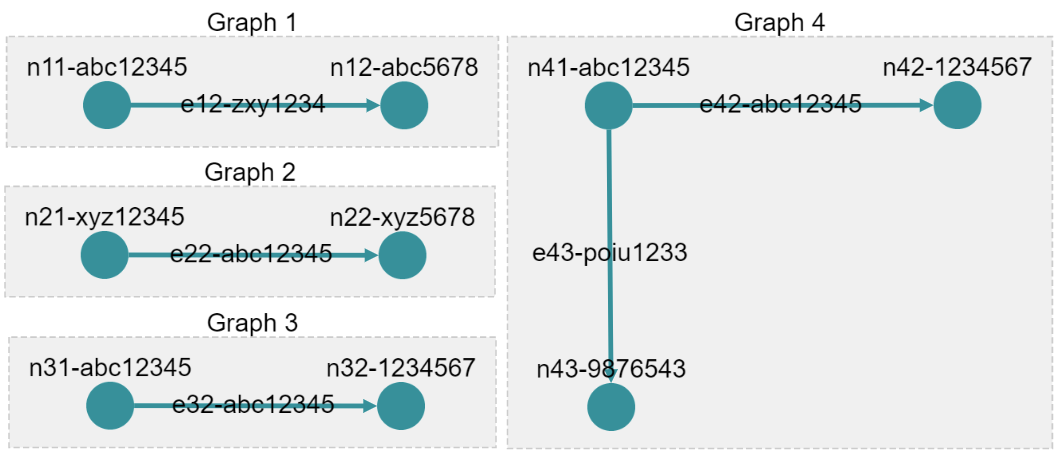
\includegraphics[scale=0.6]{images/6-TestGraphs.png}
\captionof{figure}{Test graphs used for testing. The circle represents an abstract state, and the line represents the abstract actions between the abstract states}\label{fig:test-graphs}
\endgroup

Each scenario follows the same pattern. The first two graphs from the background are chosen and set as either the old or new. Then the comparison is run, and the comparison result is merged. After the merge, the actual result is asserted with the validation described. Five scenarios are tested using this pattern, divided into four specific tests focusing on a specific qualification of a change. The fifth scenario is a more extensive test representing the experiment application discussed in the next section.

\todo{Add more information about experiment}

The four specific tests are as follows (1) validation that the initial states are recognised as corresponding states, (2) Going from a corresponding state, following action with the same id, validating that the target state is recognised as corresponding states, (3) When a new abstract state is added validate it is recognised and merge as such, (4) When an abstract state is removed in the new version validate it is recognised and merged as such.

The fifth scenario used two different graphs, which are visualised in figure \ref{fig:bigger-test-graphs}. The graphs both have the same initial state, going to an intermediate state where actions v1, v2 and v3 can be executed. In graph six, the v3 action has been added, and the v1 action is removed. A merge graph is generated by running the scenario, which is visualised in figure \ref{fig:test-merged-graph}. The merge graph is what was expected. 

\begingroup
\captionsetup{type=figure}
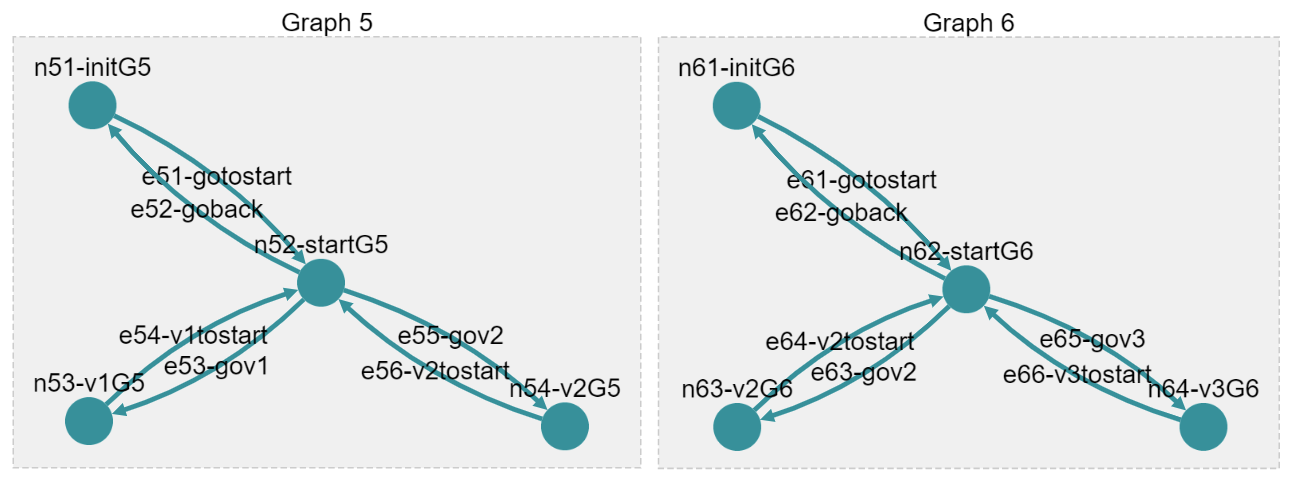
\includegraphics[scale=0.5]{images/6-test-graph-5-6.png}
\captionof{figure}{Graphs 5 and 6 for the bigger scenario. The circle represents an abstract state. The line represents the abstract actions between the abstract states}\label{fig:bigger-test-graphs}
\endgroup

The merge graph uses different colours and shapes to indicate removed and added states. Using an alternative form of representing the outcome, besides colours, makes it possible to distinguish normal, removed or added states even when the results are printed in black-and-white or with people who are colour blind. A red triangle represents a removed abstract state. A green star indicates a new abstract state.

\begingroup
\captionsetup{type=figure}
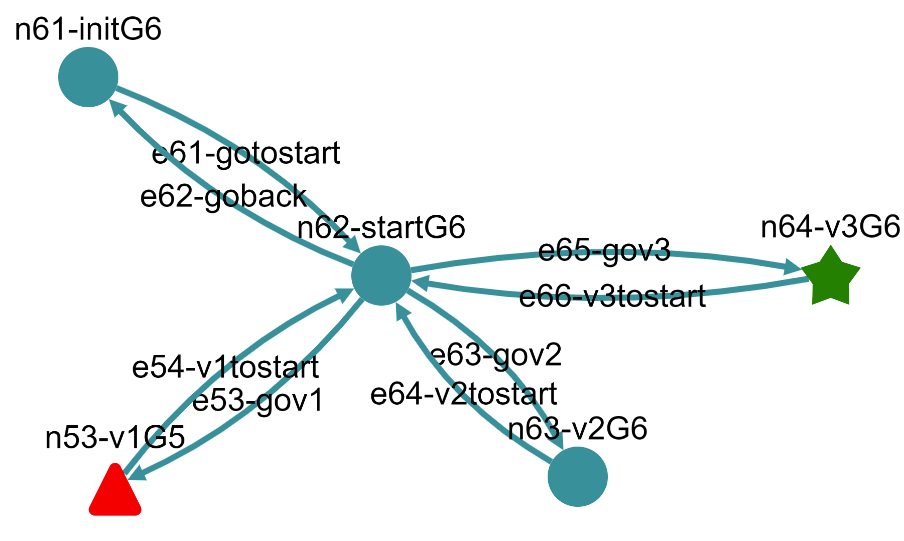
\includegraphics[scale=0.5]{images/6-merge-result.png}
\captionof{figure}{The merge result is visualised. The circle represents an abstract state, a green star represents a new and, the red triangle represents a removed abstract state, and the line represents the abstract actions between the abstract states }\label{fig:test-merged-graph}
\endgroup


\subsection{Outcome of the technical tests}
By running the scenario, one issue was found in the merge engine. Section \ref{sec:merge-graph} explains that the edged (abstract actions in \testar case) must be rewired from the old graph to the merge graph. Adding all the old edges led to duplication of actions since corresponding actions were already present in the merge graph. The issue was fixed by keeping track of the action id while making the merge graph. When an action already existed in the set of action Id, the action was skipped for rewiring. 

\section{Experimental application} \label{sec:experimental-application}

\subsection{The application}

The application under test is an application created in .NET. The source code can be found in the companion GitHub repository \footnote{\url{https://github.com/rneeft/study-ga/tree/main/experiment/TestarChangeDetectionExperiment}}. The application is an upgraded two-button application mentioned in section \ref{sec:state-model-difference}. Figure \ref{fig:experiment-start} shows the start screen of the experiment application whereas figures \ref{fig:experiment-v1}, \ref{fig:experiment-v2} and \ref{fig:experiment-v2}  shows the three different versions. The start screen is added, and the back button enables going back to ensure the initial state of all the applications is equal. 

\begin{tabularx}{\textwidth}{@{} 
   >{\raggedright\arraybackslash}X
   >{\raggedright\arraybackslash}X  }
    \begingroup
    \captionsetup{type=figure}
    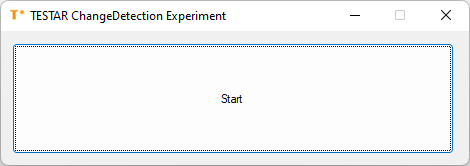
\includegraphics[scale=0.60]{images/6-Experiment-Start.png}
    \captionof{figure}{Start screen}\label{fig:experiment-start}
    \endgroup
    &
    \begingroup
    \captionsetup{type=figure}
    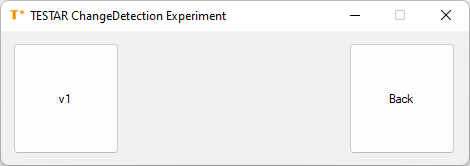
\includegraphics[scale=0.60]{images/6-Experiment-v1.png}
    \captionof{figure}{Version 1}\label{fig:experiment-v1}
    \endgroup
    
    \\
    
    \begingroup
    \captionsetup{type=figure}
    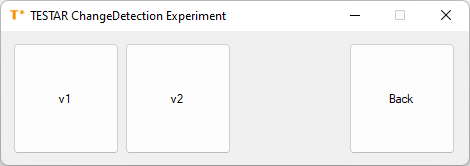
\includegraphics[scale=0.6]{images/6-Experiment-v2.png}
    \captionof{figure}{Version 2}\label{fig:experiment-v2}
    \endgroup
    &
    \begingroup
    \captionsetup{type=figure}
    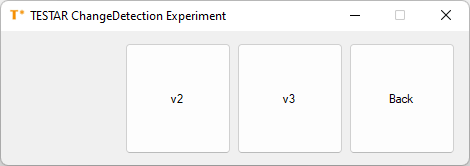
\includegraphics[scale=0.6]{images/6-Experiment-v3.png}
    \captionof{figure}{Version 3}\label{fig:experiment-v3}
    \endgroup
\end{tabularx}

The changes can be observed in the figures above, version 2 has a new v2 button and in version 3 the v3 button is added and the v1 button is removed. When clicking on the buttons a message screen appears with the following text: 'Hello world version 1' for the v1 button, 'Welcome to version 2' for the v2 button and 'This is version 3!!' for the v3 button. The Back button brings the application back to the start screen in figure \ref{fig:experiment-start}. 

\subsection{Generating models}
All three versions are compiled into one single executable. Selecting a version during the executable's startup is done by supplying an argument. For example, to start the application in version 2 use the command \verb|Experiment.exe v2|. It is possible to start the application without the start screen by adding the argument \verb|-nostart|. The application will not show the start and the \textit{Back} button. 

The application was tested with the \testar default protocol \verb|desktop_generic_statemodel|. In the \testar analysis screen (figure \ref{fig:advance}) the 'widget title' is selected for creating the abstract model.  The three abstract layers generated by \testar are displayed in figure \ref{fig:abstract-layer-default-protocol}. Although graph between version 2 and version 3 share the same structure, its has the discussed changes.

\begingroup
\captionsetup{type=figure}
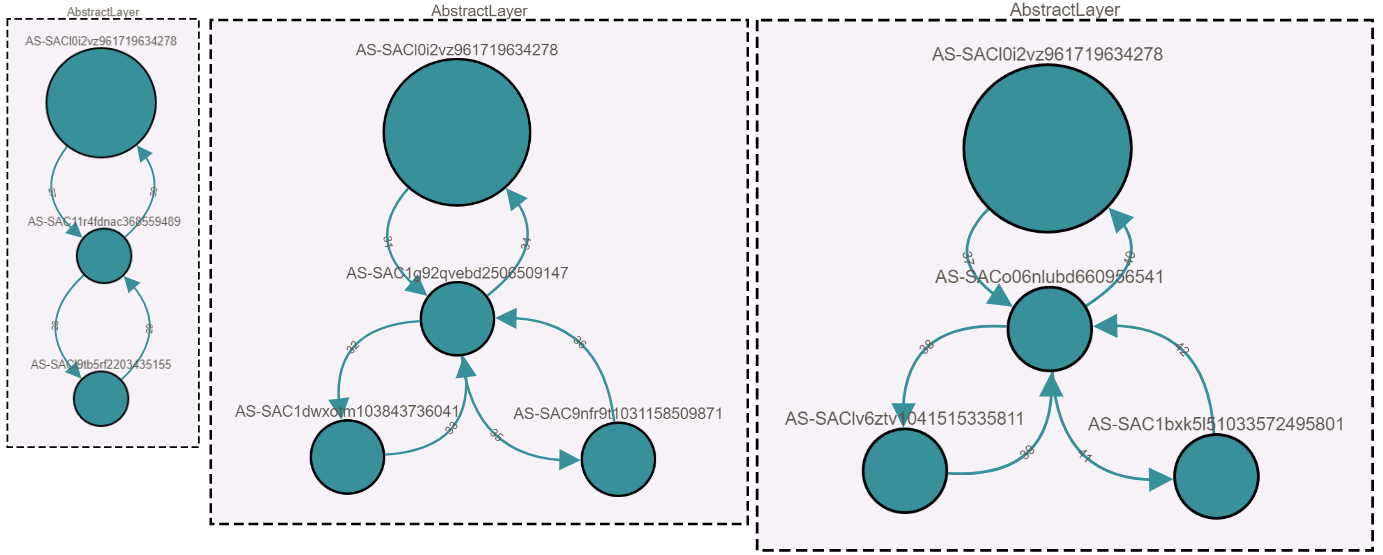
\includegraphics[scale=0.45]{images/6-Default-Protocol-Abstract-Layer.png}
\captionof{figure}{Version 1, 2 and 3 of the Experiment Application in the default protocol}\label{fig:abstract-layer-default-protocol}
\endgroup

The comparison is run between versions 2 and 1, and versions 3 and 2. The results of the two merge graphs are displayed in figure \ref{fig:wrong-merge-outcome}. The left graph is the difference between version 2 and 1, the right graph is the result of version 3 and 2. The result is not as expected but the comparison and merge are technically correct. Observing the left figure shows one removal of state and two added states. However when observing the application under test (figure \ref{fig:experiment-v1} and \ref{fig:experiment-v2}) the only change is the addition of the 'v2' button and a corresponding message. Therefor the only expected change is the one new state. 

\subsection{Non-deterministic abstract action Ids issue}

Observing the merge graph, especially the right graph, shows that two states are removed and two states are added however, between version 3 and 2 it is expected to see one state added (the v3 button) and one state removed (the v1 button).

\begingroup
\captionsetup{type=figure}
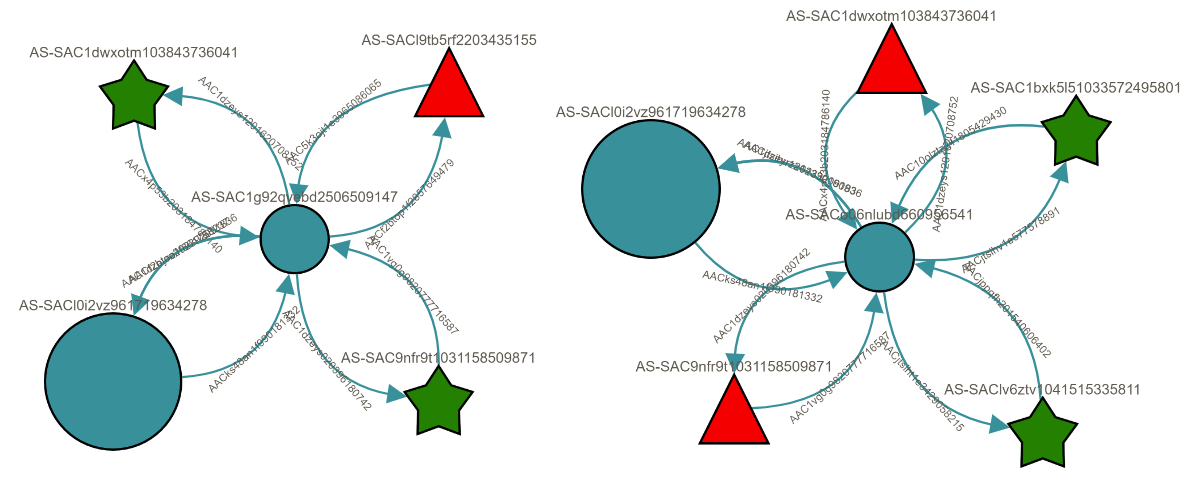
\includegraphics[scale=0.5]{images/6-Wrong-merge.png}
\captionof{figure}{Comparison outcome of the first test run}\label{fig:wrong-merge-outcome}
\endgroup

The change detection algorithm uses the \textit{action id} to find corresponding states. Observing the abstract layers of versions 1 and 2, it becomes appeared that the action Id from the initial state to the intermediate state (the state with all the buttons) is the same between the versions but that all the other action id are different, even from the intermediate state back to the initial state. It is important for the change detection algorithm to have deterministic action id over versions. 

The only selected attribute selected for the calculation of the abstract model is the 'widget title'. However the application code for calculating the action id (AbstractIDCustom in \testar) also includes the parent state in the calculation of the abstract model.

The code responsible for the calculation is found in the \verb|org.testar.monkey.DefaultProtocol| class in the method \verb|buildStateActionsIdentifiers| \footnote{\url{https://github.com/TESTARtool/TESTAR_dev/blob/db06203a54676260de5565be1ad2af026db6e969/testar/src/org/testar/monkey/DefaultProtocol.java##L1891-L1893}} which uses the \verb|buildID| method of the \\ \verb|org.testar.CodingManager| class \footnote{\url{https://github.com/TESTARtool/TESTAR_dev/blob/master/core/src/org/testar/CodingManager.java##L187-L221}}. Line 218 shows that the \verb|AbstractIDCustom| from the state is used to calculate the action id. Since the state does change between versions so does the action id. This behavior can be changed by custom code that overrides the behavior. 

\subsection{Deterministic action ids between versions}

For the detection algorithm it is very important that the action id are the same between two versions, otherwise the algorithm believes the action is either removed or added. To influence the abstract model generation behavior it is possible to change the \testar protocol. 

Listing \ref{code:protocol-changes} shows an override method for building the action id identifiers. First, the action identifiers are generated by using the default \testar code however on line 9 \& 10 the AbstractIDCustom is changed to the onenotewidget title. This change is specific to the experiment application. For other application different tags can be used but the tester needs to be sure to get deterministic action ids between versions. The full updated protocol can be found in appendix \ref{appendix:protocol-experiment}. The method \verb|lowCollisionId| is taken from the \verb|CodingManager|\footnote{\url{https://github.com/TESTARtool/TESTAR_dev/blob/db06203a54676260de5565be1ad2af026db6e969/core/src/org/testar/CodingManager.java##L301-L311}} since the access modifier is private.

\begin{lstlisting}[language=Java, caption=overwrite buildStateActionsIdentifiers method, label=code:protocol-changes]
@Override
protected void buildStateActionsIdentifiers(State state, Set<Action> actions) {
	CodingManager.buildIDs(state, actions);
	// Custom the Action AbstractIDCustom identifier
	for(Action a : actions) {
		if(a.get(Tags.OriginWidget) != null) {
			Widget widget = a.get(Tags.OriginWidget);
			// set the identifier to only containing the title and not to include the parent
			String widgetTitle = widget.get(Tags.Title);
			String customIdentifier = CodingManager.ID_PREFIX_ACTION + CodingManager.ID_PREFIX_ABSTRACT_CUSTOM + lowCollisionID(widgetTitle);
			a.set(Tags.AbstractIDCustom, customIdentifier);
		}
	}
}
\end{lstlisting}

With the new protocol the application is retested by \testar and three models are regenerate and the comparison between version 2 and 1 and versions 3 and 2 are run again. 

\begingroup
\captionsetup{type=figure}
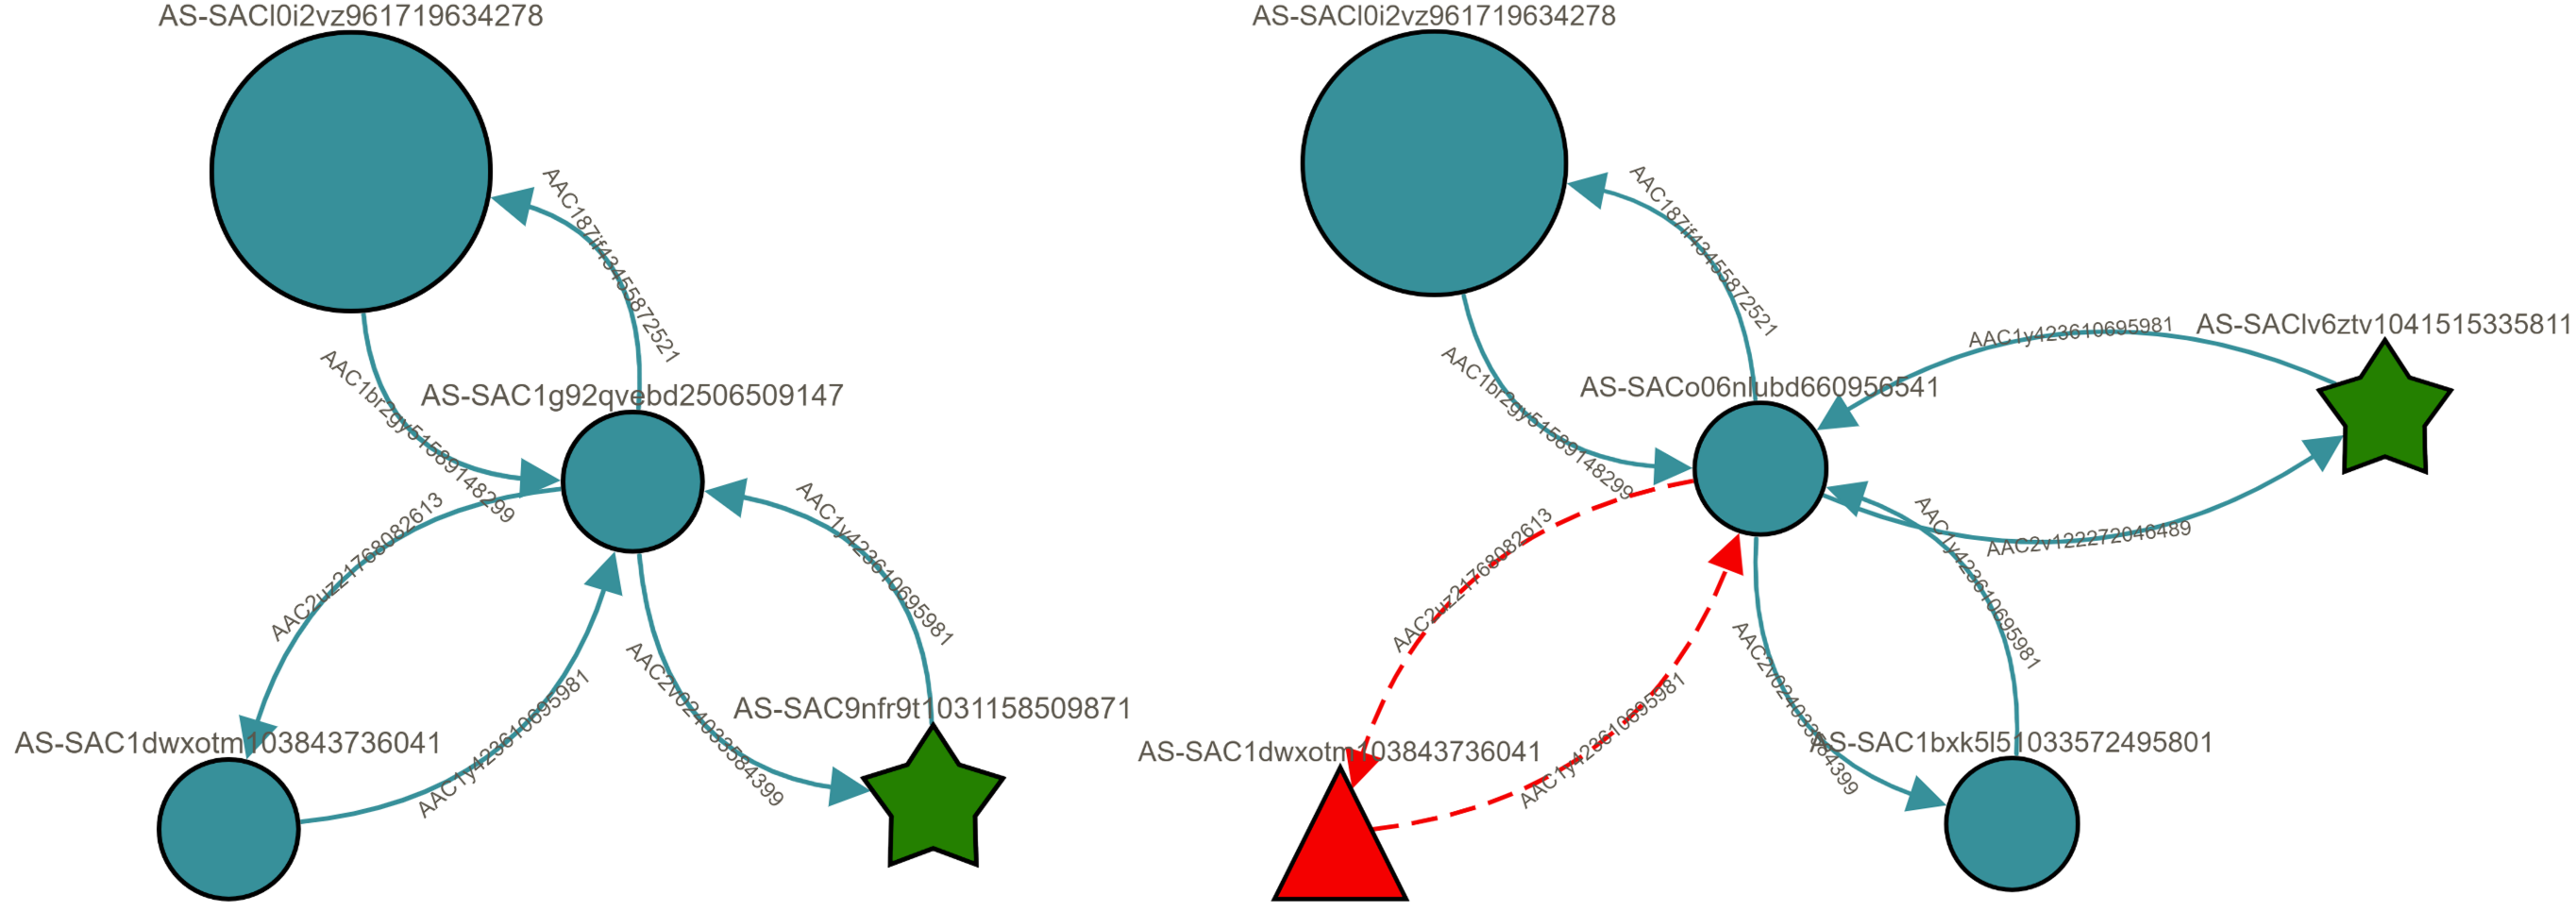
\includegraphics[scale=0.2]{images/6-Correct-Merge.png}
\captionof{figure}{Comparison outcome with updated protocol}\label{fig:correct-merge-outcome}
\endgroup

\subsection{Results and improvements}
Figure \ref{fig:correct-merge-outcome} shows the current version of the comparison and merge outcome. The section discussed the two changes that happened to get to this version.

\subsubsection{Actions id issue}
During technical testing an issue was fixed that made sure the merge graph contains no duplicated action. This was solved by keeping track of the action id that were added to the merge graph, and block actions to be added that were already added.

The experiment application showed that this resulted in states without actions. This happened because some (unrelated) action has the same action id and was therefore not added. The code was changed to not only keep track of the id of the action, but also to include the target and source identifiers.  

\subsubsection{Not clear what changed in a state}
The screenshots or data inside a corresponding state could have changed but this was not clear in the details screen. To help showing possible differences between corresponding state, the details window will show screenshots of the two states. 

In a future release it can be possible to create a pixel by pixel comparison but as of now this options was not implemented by out of the box libraries. \\

\begingroup
\captionsetup{type=figure}
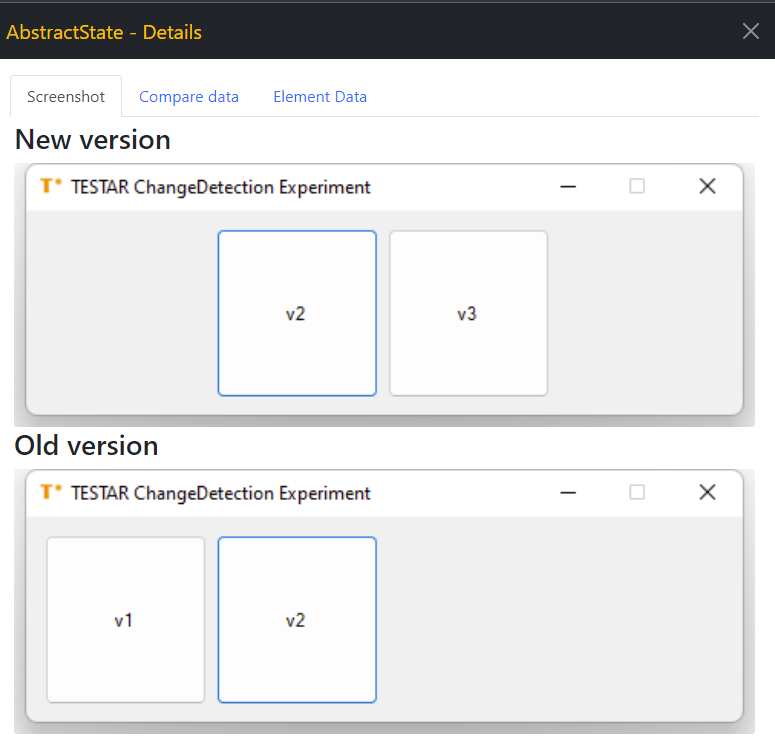
\includegraphics[scale=0.5]{images/6-Screenshot-Side-By-Side.png}
\captionof{figure}{Screenshot of corresponding states side by side}\label{fig:screenshots-side-by-side}
\endgroup